\documentclass[11pt, english, twoside]{article}
\usepackage[style=authoryear, autocite=inline, maxcitenames=3, maxbibnames=3, uniquename=false, backend=biber]{biblatex}
\usepackage[utf8]{inputenc}
\usepackage{fancyhdr}
\usepackage{graphicx}
\usepackage[onehalfspacing]{setspace}

% Customize Inline Citation Format
\renewcommand*{\finalnamedelim}{/} % Change "and" to "/"
\renewcommand*{\multinamedelim}{/} % Change ", " to "/"

% Define Custom Citation Commands
\newcommand{\vglcite}[2][]{(vgl. \cite[#1]{#2})}
\newcommand{\directcite}[2][]{(\cite[#1]{#2})}

% Customize Name Formatting in Bibliography
% \DeclareNameAlias{author}{family-given} % Ensure "Last, First" format

% % Remove ISBN, pages and series
% \AtEveryBibitem{
%   \clearfield{isbn}
%   \clearfield{pagetotal}
%   \clearfield{series}
% }

% % Customize Bibliography Author Format
% \renewbibmacro*{author}{%
%   \printnames{author}: 
% }

% \renewbibmacro*{publisher+location+date}{%
%   \printlist{location}:
%   \iflistundef{publisher}
%     {}
%     {\setunit*{\addspace}\printlist{publisher}}%
%   \setunit*{\addspace}%
%   \printfield{year}
% }

% Load Bibliography
\addbibresource{citations.bib}
\graphicspath{{images}}

% Customize Page Style
\pagestyle{fancy}
\fancyhf{}
\fancyhead[LE, LO]{\leftmark}
\fancyfoot[RE, RO]{Page \thepage}
\onehalfspacing


\begin{document}
Hello World!

% \begin{figure}[h!]
% \begin{center}
%     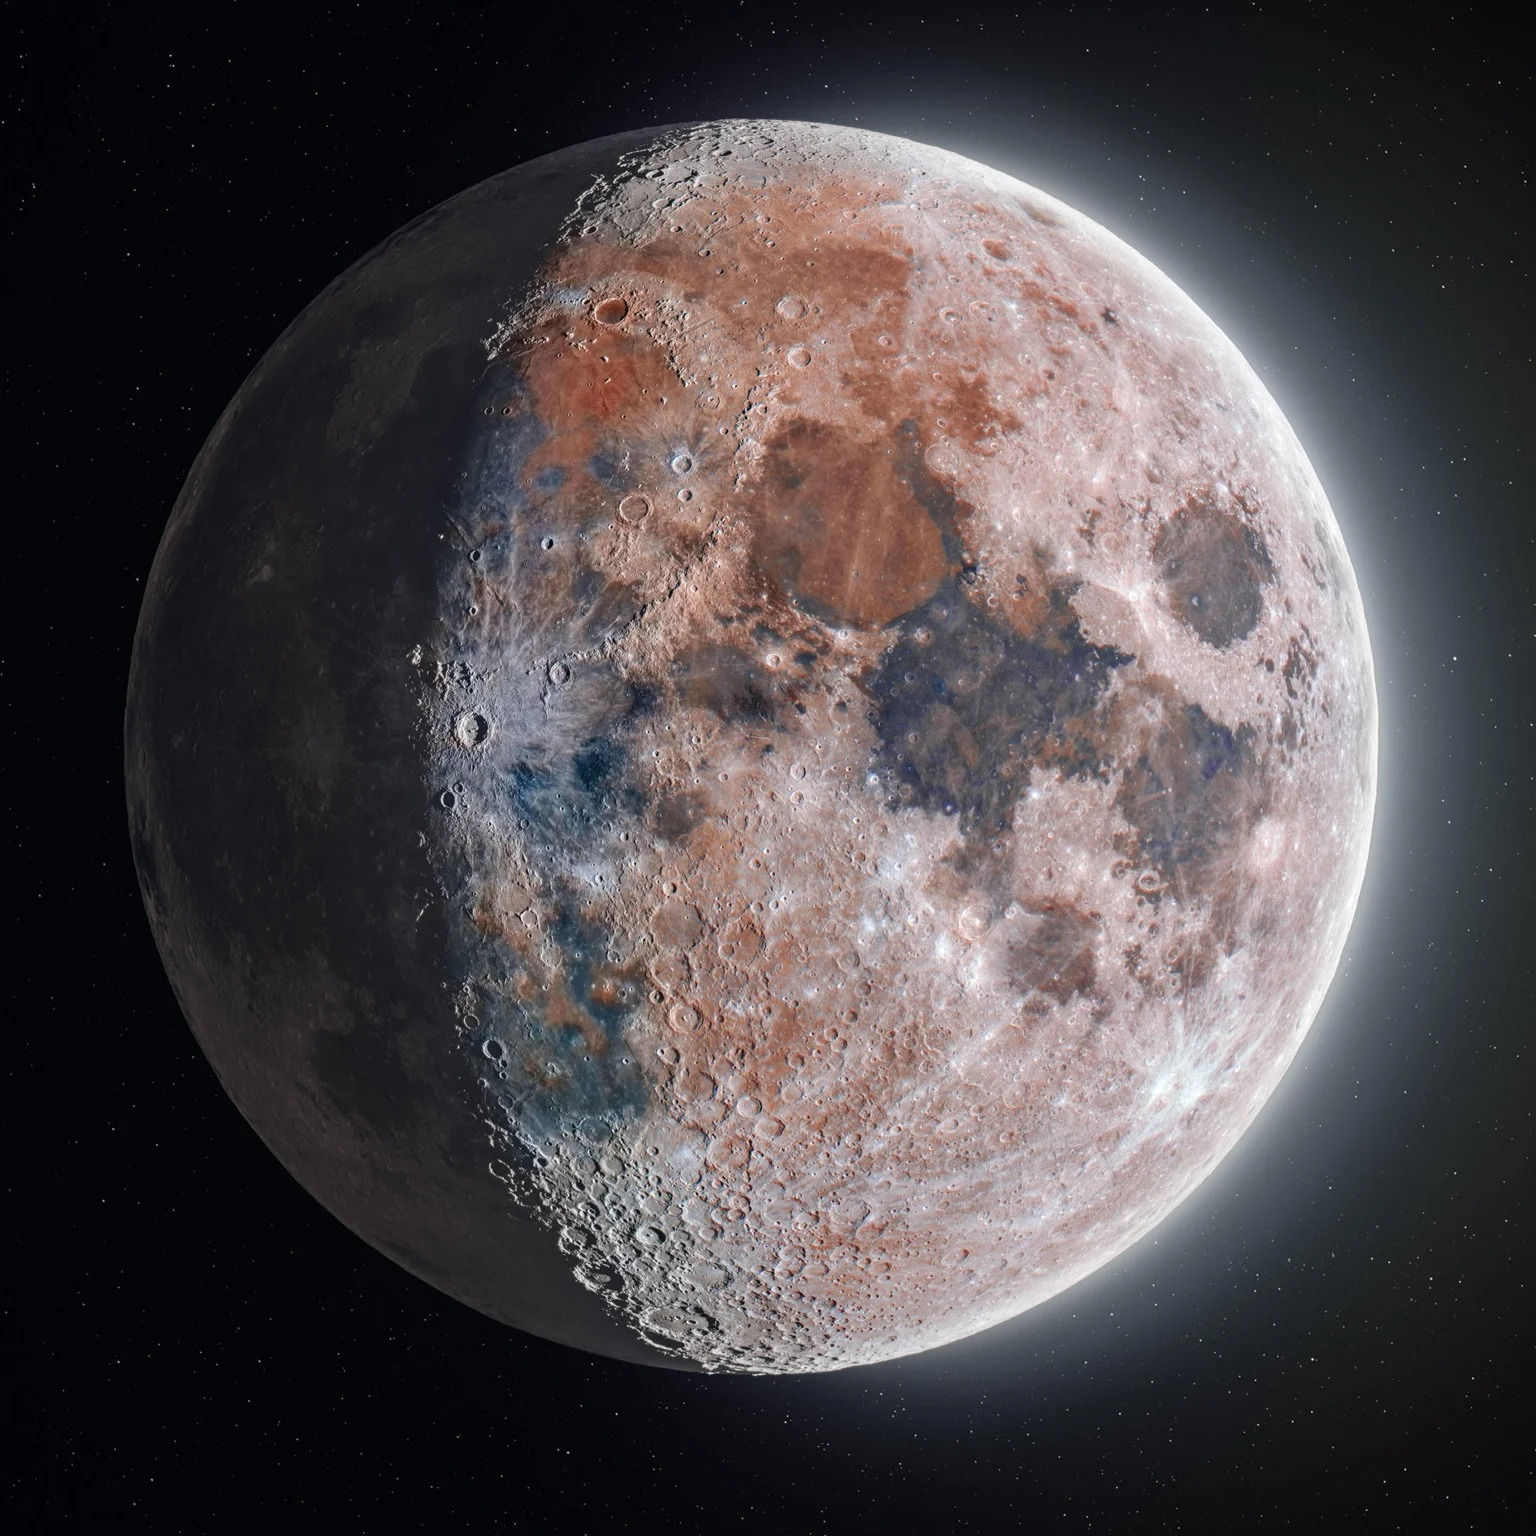
\includegraphics[width=300pt, height=\textheight,keepaspectratio]{test.jpg}
%     \caption[Caption (url)]{Caption visible}
% \end{center}
% \end{figure}

% =============== CHAPTERS ===============
\section{Introduction}


\newpage
\section{Basics of Webdesign}
Optimizing the workflow from User Interface Design to code implementation requires to have a solid
foundational understanding of what UI Design and development is. More specifically, understanding
web-specific aspects of these fields is crucial to optimize the workflow for web projects. In this
chapter, we will discuss the basics of User Interface Design.

\newpage
\subsection{User Interface Design}
The interaction design foundation defines User Interface (UI) Design as "the process designers use
to build interfaces in software or computerized devices, focusing on looks or style. Designers aim
to create interfaces which users find easy to use and pleasurable. UI design refers to graphical
user interfaces and other forms—e.g., voice-controlled interfaces."
\directcite{interactiondesignfoundation-ixdfWhatUserInterface2016}.

This definition is a good starting point to understand what UI design is about, since it
shows that it is about more than just the visual. User interfaces are everywhere, be it an ATM, a
stove, a bike computer or a time tracking app in the browser. Each one of them needs to be
carefully designed. It is about finding ways to make this human-computer interaction as smooth,
efficient and delightful as possible.
\vglcite{interactiondesignfoundation-ixdfWhatUserInterface2016}

\subsubsection{Web Design}
Web Design is a subset of UI Design that specifically focuses on designing websites. While other UI
Design fields often focus on specific platforms, web designers have to consider a wide range of end
user devices like desktop PCs, tablets or smartphones. The practice of adapting and optimizing for
these various screen sizes and aspect ratios is known as \textit{Responsive Design}. Additionally,
\textit{Web Accessibility} is a fundamental aspect of Web Design. It ensures that people with
disabilities can navigate and interact with websites as effectively as possible.
\vglcite{interactiondesignfoundation-ixdfWhatWebDesign2016}

With the European Accessibility Act (EAA) coming into effect in June 2025, this becomes even more
important, as businesses need to comply with stricter regulations on all of their websites.
\vglcite{kleeAccessibilityAct20252024}

Although Web Design is often thought of as a purely visual discipline, when in reality it is a much
more multidisciplinary field. They have to work closely with developers and often know a great deal
of content strategy, information architecture, user research and more. Product designer Mark Boulton
emphazises that "You can create good experiences without knowing the content. What you can’t do is
create good experiences without knowing your content structure. What is your content made from, not
what your content is." \directcite[]{boultonStructureFirstContent2012}

\subsubsection{User Experience and Usability}
Zooming out of the context of User Interfaces is essential to fully understand the concept of User
Experience (UX). UX is about looking at all kinds of touchpoints a user has with a product or
service and seeing the holistic experience. This of course includes the UI, but encompasses several
other domains such as content quality, customer support, branding, and more.
\vglcite{normanDefinitionUserExperience1998}

In other words, even an app like Spotify with a great interface, would have a poor UX if there were
only 10 songs available.

Usability on the other hand is, as Jacob Nielsen suggests, a quality attribute of Interfaces. This
attribute indicates how easy it is for users to use a product, by observing and measuring the five
quality components: learnability, efficiency, memorability, errors, and satisfaction
defined by Nielsen. Additionally, Nielsen introduces another concept that when combined with
usability is an indicator for the overall usefulness of a product - utility. Utility refers to
whether a product offers the necessary features that a user actually needs. Both usability and
utility are crucial for a successful product. Simply having an intuitive interface is of no use if
the product lacks the necessary features, similarly, a product with a fitting feature-set is
ineffective if users struggle navigating it.
\vglcite{nielsenUsability101Introduction2012}
% NOTE DONE: Potential for graphic here (Vann Diagram)
\begin{figure}[H]
    \centering
    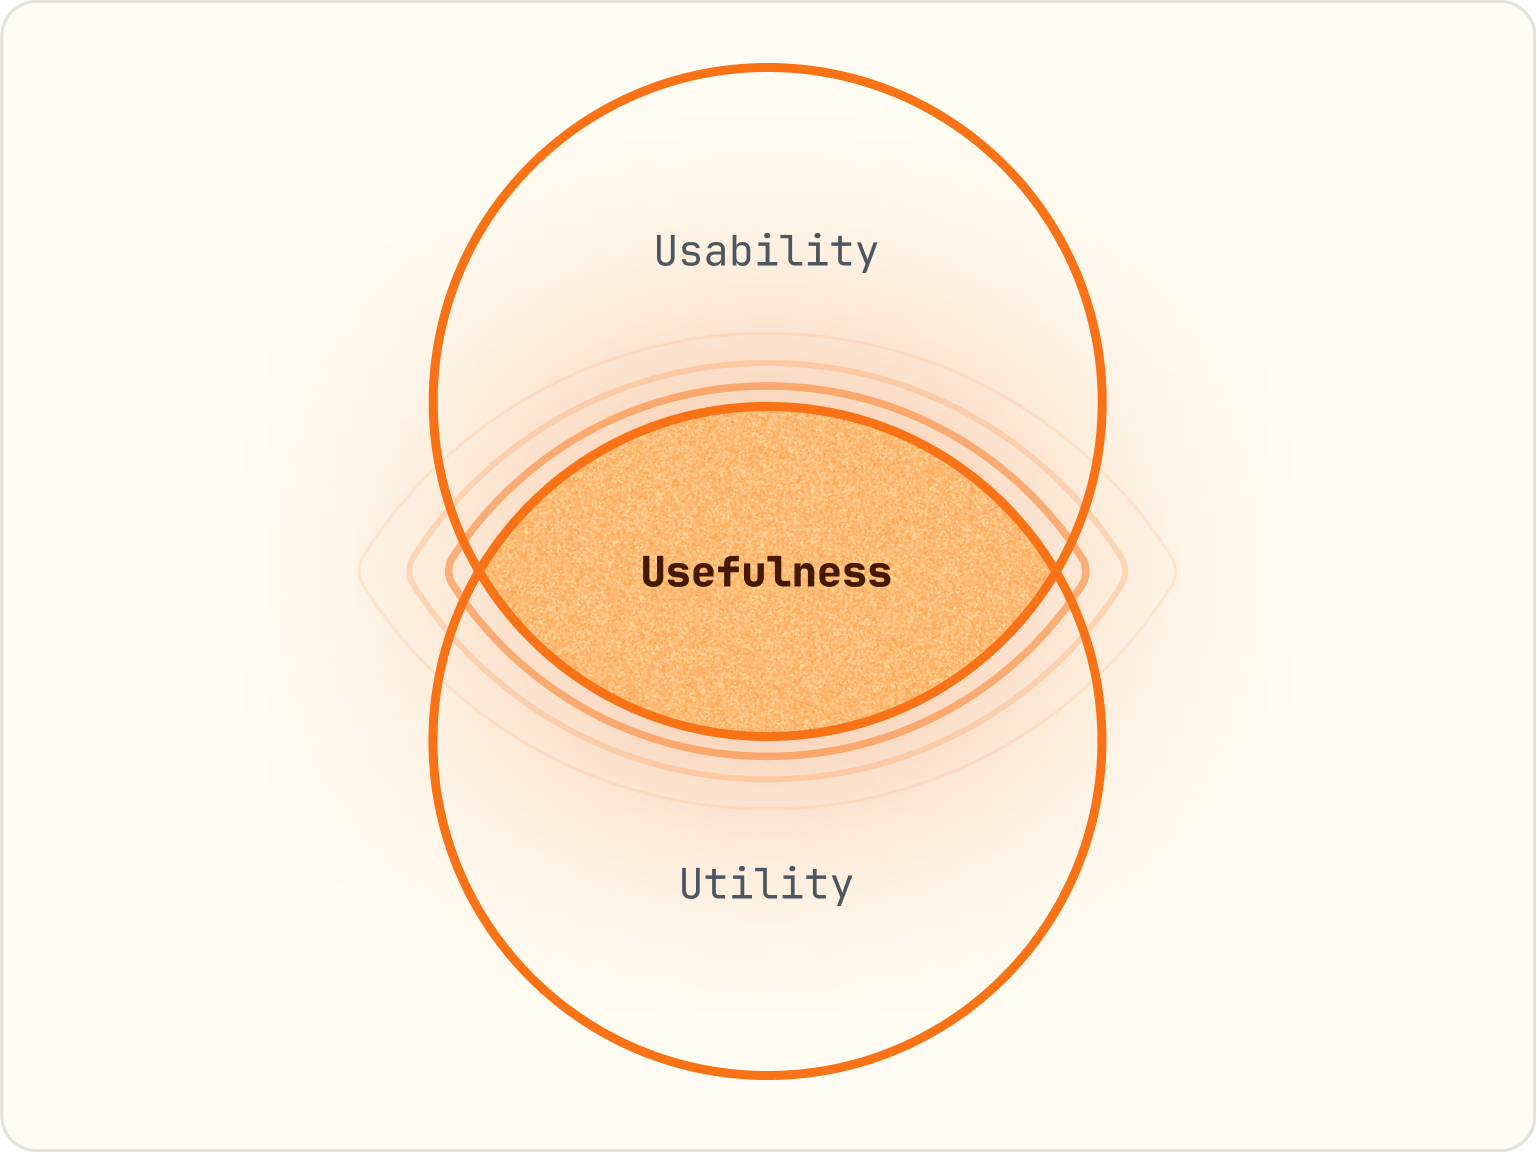
\includegraphics[height=250pt]{Chapter 2/Usefulness.png}
    \caption{Combination of usability and utility according to Jacob Nielsen (Source: own illustration)}
\end{figure}

\subsubsection{Tools}
There are many great tools available that aim to make User Interface Design easier and more
efficient. Some of them also have features that help to bridge the gap between design and code. The
selection of tools is based on their popularity, since the aim is to provide a solution that
tailors to the majority of designers and developers. % NOTE DONE: Add graphic showing the popularity of
% tools (https://uxtools.co/survey/2023/ui-design/#ui-design-yoy-graph)

% NOTE DONE: Add Logo graphic for each of the tools
\textbf{Figma}\\
\begin{figure}[H]
    
\includegraphics[height=50pt]{Chapter 2/Figma.png}
    \caption{Figma Logo (Source: modified illustration based on Figma in https://www.figma.com/using-the-figma-brand/)}
\end{figure}
According to UXTools yearly survey, Figma is by far the most popular UI Design tool at the moment.
\vglcite{uxtools2024DesignTools2024} It is a cloud-based design tool that focuses on real-time
collaboration, prototyping and design system creation. The majority of features is free to use,
which makes it very approachable. Apart from their frequent updates and improvements, Figma has a
lively community allowing for the creation of plugins, templates and other resources. Having robust
design system features like components, style definitions and variables, Figma is one of the leading
tools in the UI Design space. \vglcite{figmaFigma}

\textbf{Sketch}\\
\begin{figure}[H]
    
\includegraphics[height=50pt]{Chapter 2/Sketch.png}
    \caption{Sketch Logo (Source: modified illustration based on Sketch in https://www.sketch.com/about-us)}
\end{figure}
Sketch: Sketch is a design tool that was first released in 2010. Although, Figma has surpassed
Sketch in popularity, it still has a large user base. It offers similar features to Figma like
real-time collaboration, components or prototyping. However, aside from the free, browser-accessible
file viewer, Sketch is a paid tool available only on macOS. The program has a strong focus on
creating design systems and a large library of available plugins and templates.
\vglcite{sketchSketch}

\textbf{Adobe Illustrator and Adobe Photoshop}\\
\begin{figure}[H]
    
\includegraphics[height=50pt]{Chapter 2/Illustrator.png}
    \caption{Illustrator Logo (Source: modified illustration based on Adobe in https://www.adobe.com/cc-shared/assets/img/product-icons/svg/illustrator.svg)}
\end{figure}
Although the vector graphics editor Adobe Illustrator and the raster graphics editor Adobe Photoshop
are not specifically tailored to UI Design, they are widely used by designers. Many designers report
that they use them as secondary tools aiding in the creation of more complex graphics.
\vglcite{uxtools2024DesignTools2024}

In future chapters, I will generally refer to Figma, since it is the most popular tool at the moment
and also the one I am most familiar with. Although the majority of concepts and techniques mentioned
will be applicable to other tools as well.


\newpage
\subsection{Component Based UI Design}
UI Designs without realising them through code are similar to having a blueprint for a house. They
provide a detailed plan of how the final product should look like and function, but remain mostly
nonfunctional on their own. Similarly, engineers rely on these blueprints to bring the vision to
life. It is the collaboration of the two disciplines that result in a building, or in this case, a
website. UI Design depends on development and vice versa. 

Because of this strong dependency, it only makes sense that both disciplines share common concepts
and principles. One of these concepts is called Component Based Design.

\subsubsection{The Concept of Components}
This concept originates from a programming paradigm called Component Based Software Engineering
(CBSE). Without getting too much into the technical details, CBSE is about breaking down software
into smaller, independent and reusable parts called components. This modularity allows for easier
maintenance, scalability and reliability of code.
\vglcite[20,22]{tiwariCOMPONENTBASEDSOFTWAREENGINEERING2024}

I mention this specifically, since it is a core principle of modern web development and UI Design.
After the release of Angular in 2010, this concept started really gaining traction in web
development. \vglcite{angularjsAngularJS}
% NOTE: Maybe say that in 2013 Atomic Design was introduced by Brad Frost and got UI Design on board
Now, almost all popular frontend frameworks like React, Vue or Svelte are built around components.
\vglcite{reactReact} \vglcite{vuejsVueJS} \vglcite{svelteSvelte}

Around the same time as Component Based Design became popular in web development, Brad Frost
introduced Atomic Design, which translates this programming concept to UI Design. In section
\ref{Atomic Design Systems}, the concept of Atomic Design and how it can be used practically will be
explored in more detail. Essentially Frost took chemistry as an inspiration and composed a methodology
using five stages called Atoms, Molecules, Organisms, Templates and Pages that should serve as a
\textit{mental model} for UI Designers. \vglcite[42]{frostAtomicDesign2016}

Today, Component Based UI Design is a deep rooted part of almost every Interface Design tool as
well. That is why it is incredibly crucial for designers to understand this concept and how it can
be effectively applied to their work. Since, in theory, this approach brings design and development
closer to the ideal of seamless collaboration, resulting in interfaces that are both beautiful,
functional, and maintainable.

\subsection{Design Systems}
\subsubsection{Parts of the Design System}
% Just explain the parts: 
% - Style Guide
% - Pattern Library
% - Component Library
% - Design Tokens
\subsubsection{Common Best Practices for Design Systems}

\newpage
\subsection{User Interface Design}
The interaction design foundation defines User Interface (UI) Design as "the process designers use
to build interfaces in software or computerized devices, focusing on looks or style. Designers aim
to create interfaces which users find easy to use and pleasurable. UI design refers to graphical
user interfaces and other forms—e.g., voice-controlled interfaces."
\directcite{interactiondesignfoundation-ixdfWhatUserInterface2016}.

This definition is a good starting point to understand what UI design is about, since it
shows that it is about more than just the visual. User interfaces are everywhere, be it an ATM, a
stove, a bike computer or a time tracking app in the browser. Each one of them needs to be
carefully designed. It is about finding ways to make this human-computer interaction as smooth,
efficient and delightful as possible.
\vglcite{interactiondesignfoundation-ixdfWhatUserInterface2016}

\subsubsection{Web Design}
Web Design is a subset of UI Design that specifically focuses on designing websites. While other UI
Design fields often focus on specific platforms, web designers have to consider a wide range of end
user devices like desktop PCs, tablets or smartphones. The practice of adapting and optimizing for
these various screen sizes and aspect ratios is known as \textit{Responsive Design}. Additionally,
\textit{Web Accessibility} is a fundamental aspect of Web Design. It ensures that people with
disabilities can navigate and interact with websites as effectively as possible.
\vglcite{interactiondesignfoundation-ixdfWhatWebDesign2016}

With the European Accessibility Act (EAA) coming into effect in June 2025, this becomes even more
important, as businesses need to comply with stricter regulations on all of their websites.
\vglcite{kleeAccessibilityAct20252024}

Although Web Design is often thought of as a purely visual discipline, when in reality it is a much
more multidisciplinary field. They have to work closely with developers and often know a great deal
of content strategy, information architecture, user research and more. Product designer Mark Boulton
emphazises that "You can create good experiences without knowing the content. What you can’t do is
create good experiences without knowing your content structure. What is your content made from, not
what your content is." \directcite[]{boultonStructureFirstContent2012}

\subsubsection{User Experience and Usability}
Zooming out of the context of User Interfaces is essential to fully understand the concept of User
Experience (UX). UX is about looking at all kinds of touchpoints a user has with a product or
service and seeing the holistic experience. This of course includes the UI, but encompasses several
other domains such as content quality, customer support, branding, and more.
\vglcite{normanDefinitionUserExperience1998}

In other words, even an app like Spotify with a great interface, would have a poor UX if there were
only 10 songs available.

Usability on the other hand is, as Jacob Nielsen suggests, a quality attribute of Interfaces. This
attribute indicates how easy it is for users to use a product, by observing and measuring the five
quality components: learnability, efficiency, memorability, errors, and satisfaction
defined by Nielsen. Additionally, Nielsen introduces another concept that when combined with
usability is an indicator for the overall usefulness of a product - utility. Utility refers to
whether a product offers the necessary features that a user actually needs. Both usability and
utility are crucial for a successful product. Simply having an intuitive interface is of no use if
the product lacks the necessary features, similarly, a product with a fitting feature-set is
ineffective if users struggle navigating it.
\vglcite{nielsenUsability101Introduction2012}
% NOTE DONE: Potential for graphic here (Vann Diagram)
\begin{figure}[H]
    \centering
    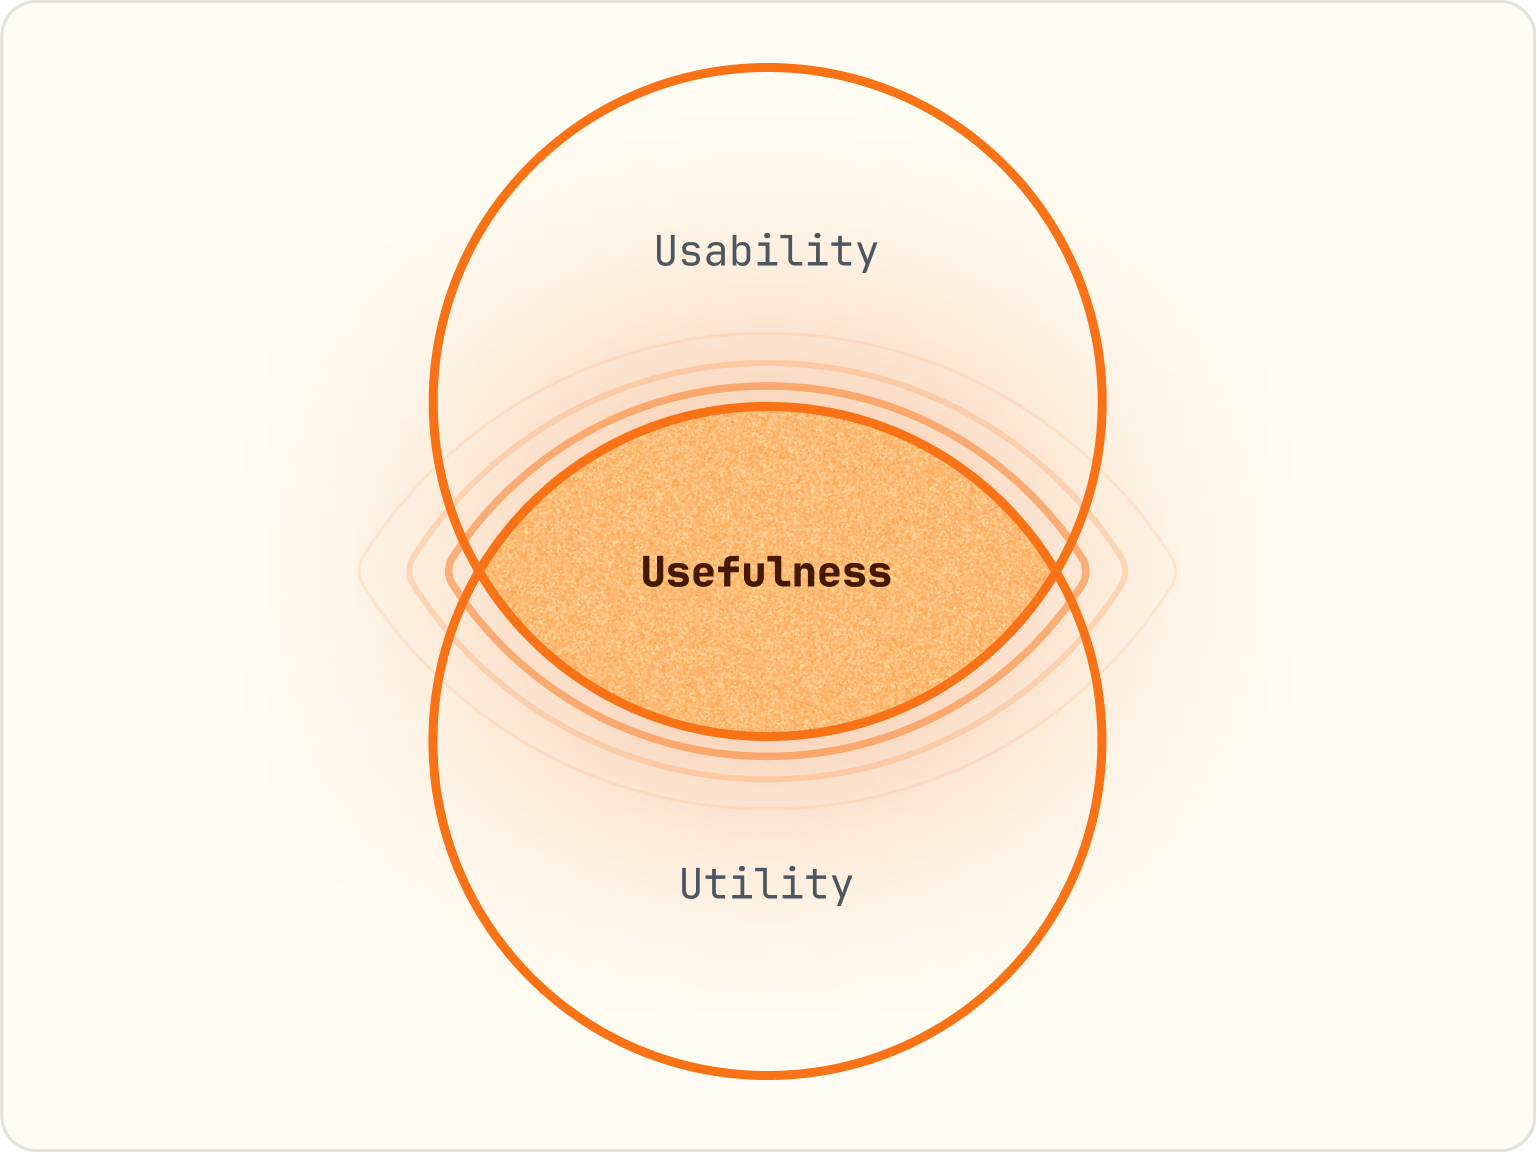
\includegraphics[height=250pt]{Chapter 2/Usefulness.png}
    \caption{Combination of usability and utility according to Jacob Nielsen (Source: own illustration)}
\end{figure}

\subsubsection{Tools}
There are many great tools available that aim to make User Interface Design easier and more
efficient. Some of them also have features that help to bridge the gap between design and code. The
selection of tools is based on their popularity, since the aim is to provide a solution that
tailors to the majority of designers and developers. % NOTE DONE: Add graphic showing the popularity of
% tools (https://uxtools.co/survey/2023/ui-design/#ui-design-yoy-graph)

% NOTE DONE: Add Logo graphic for each of the tools
\textbf{Figma}\\
\begin{figure}[H]
    
\includegraphics[height=50pt]{Chapter 2/Figma.png}
    \caption{Figma Logo (Source: modified illustration based on Figma in https://www.figma.com/using-the-figma-brand/)}
\end{figure}
According to UXTools yearly survey, Figma is by far the most popular UI Design tool at the moment.
\vglcite{uxtools2024DesignTools2024} It is a cloud-based design tool that focuses on real-time
collaboration, prototyping and design system creation. The majority of features is free to use,
which makes it very approachable. Apart from their frequent updates and improvements, Figma has a
lively community allowing for the creation of plugins, templates and other resources. Having robust
design system features like components, style definitions and variables, Figma is one of the leading
tools in the UI Design space. \vglcite{figmaFigma}

\textbf{Sketch}\\
\begin{figure}[H]
    
\includegraphics[height=50pt]{Chapter 2/Sketch.png}
    \caption{Sketch Logo (Source: modified illustration based on Sketch in https://www.sketch.com/about-us)}
\end{figure}
Sketch: Sketch is a design tool that was first released in 2010. Although, Figma has surpassed
Sketch in popularity, it still has a large user base. It offers similar features to Figma like
real-time collaboration, components or prototyping. However, aside from the free, browser-accessible
file viewer, Sketch is a paid tool available only on macOS. The program has a strong focus on
creating design systems and a large library of available plugins and templates.
\vglcite{sketchSketch}

\textbf{Adobe Illustrator and Adobe Photoshop}\\
\begin{figure}[H]
    
\includegraphics[height=50pt]{Chapter 2/Illustrator.png}
    \caption{Illustrator Logo (Source: modified illustration based on Adobe in https://www.adobe.com/cc-shared/assets/img/product-icons/svg/illustrator.svg)}
\end{figure}
Although the vector graphics editor Adobe Illustrator and the raster graphics editor Adobe Photoshop
are not specifically tailored to UI Design, they are widely used by designers. Many designers report
that they use them as secondary tools aiding in the creation of more complex graphics.
\vglcite{uxtools2024DesignTools2024}

In future chapters, I will generally refer to Figma, since it is the most popular tool at the moment
and also the one I am most familiar with. Although the majority of concepts and techniques mentioned
will be applicable to other tools as well.


\newpage
\subsection{Component Based UI Design}
UI Designs without realising them through code are similar to having a blueprint for a house. They
provide a detailed plan of how the final product should look like and function, but remain mostly
nonfunctional on their own. Similarly, engineers rely on these blueprints to bring the vision to
life. It is the collaboration of the two disciplines that result in a building, or in this case, a
website. UI Design depends on development and vice versa. 

Because of this strong dependency, it only makes sense that both disciplines share common concepts
and principles. One of these concepts is called Component Based Design.

\subsubsection{The Concept of Components}
This concept originates from a programming paradigm called Component Based Software Engineering
(CBSE). Without getting too much into the technical details, CBSE is about breaking down software
into smaller, independent and reusable parts called components. This modularity allows for easier
maintenance, scalability and reliability of code.
\vglcite[20,22]{tiwariCOMPONENTBASEDSOFTWAREENGINEERING2024}

I mention this specifically, since it is a core principle of modern web development and UI Design.
After the release of Angular in 2010, this concept started really gaining traction in web
development. \vglcite{angularjsAngularJS}
% NOTE: Maybe say that in 2013 Atomic Design was introduced by Brad Frost and got UI Design on board
Now, almost all popular frontend frameworks like React, Vue or Svelte are built around components.
\vglcite{reactReact} \vglcite{vuejsVueJS} \vglcite{svelteSvelte}

Around the same time as Component Based Design became popular in web development, Brad Frost
introduced Atomic Design, which translates this programming concept to UI Design. In section
\ref{Atomic Design Systems}, the concept of Atomic Design and how it can be used practically will be
explored in more detail. Essentially Frost took chemistry as an inspiration and composed a methodology
using five stages called Atoms, Molecules, Organisms, Templates and Pages that should serve as a
\textit{mental model} for UI Designers. \vglcite[42]{frostAtomicDesign2016}

Today, Component Based UI Design is a deep rooted part of almost every Interface Design tool as
well. That is why it is incredibly crucial for designers to understand this concept and how it can
be effectively applied to their work. Since, in theory, this approach brings design and development
closer to the ideal of seamless collaboration, resulting in interfaces that are both beautiful,
functional, and maintainable.

\subsection{Design Systems}
\subsubsection{Parts of the Design System}
% Just explain the parts: 
% - Style Guide
% - Pattern Library
% - Component Library
% - Design Tokens
\subsubsection{Common Best Practices for Design Systems}
% =============== CHAPTERS ===============



% =============== REFERENCES ===============
\newpage
\printbibliography

\newpage
\listoffigures
% =============== REFERENCES ===============
\end{document}
